\textbf{10.1.} 一电路如图 10.1 所示, 其中 L 是电感 (它的电阻可略去不计), $A_{1}$ 、 $A_{2}$ 和 $A_{3}$ 是三个小灯泡; 先接通电键 K, 电源的电压使它们都正常发光. 然后断开 K, 试问三个小灯泡哪个先熄灭? 哪个后熄灭? 为什么?


【解答】K断开后，通过 $A_{1}$ 的电流为零，故 $A_{1}$ 先熄灭，K断开后， $L$ 中的感应电动势在 $LA_{2}A_{3}$ 回路中产生的感应电流随时间 $t$ 指数下降，故 $A_{2}$ 和 $A_{3}$ 后熄灭，且 $A_{2}$ 和 $A_{3}$ 同时熄灭.
\begin{center}
    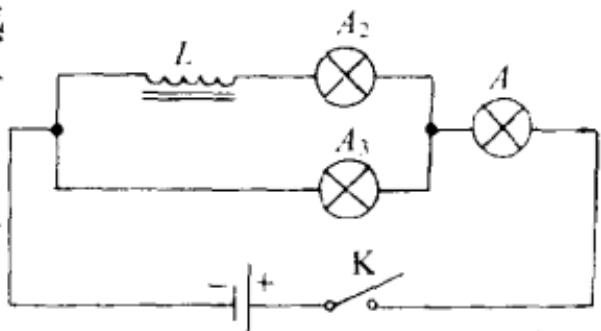
\includegraphics[width=0.5\linewidth]{figures/fig_10_1.jpg}
\end{center}

\vfill

\textbf{10.2.} 一电路如图 10.2(1)所示,其中 L 是电感(它的电阻可略去不计), $A_{1}$ 和 $A_{2}$ 是两个相同的小灯泡,电源的电压可以使它们正常发光,K 是开关.在下列两种情况下,各列出了四种现象,试问其中哪种现象是对的?(1)接通 K:(a) $A_{1}$ 先亮, $A_{2}$ 后亮;(b) $A_{2}$ 先亮, $A_{1}$ 后亮;(c) $A_{1}$ 和 $A_{2}$ 同时亮,且都一直亮下去;(d) $A_{1}$ 和 $A_{2}$ 同时亮, $A_{1}$ 随即熄灭.(2)K 接通后电流达到稳定,再断开 K:(a) $A_{1}$ 和 $A_{2}$ 同时熄灭;(b) $A_{1}$ 先熄灭, $A_{2}$ 后熄灭;(c) $A_{2}$ 先熄灭, $A_{1}$ 后熄灭;(d) $A_{2}$ 先熄灭, $A_{1}$ 突然闪亮一下然后熄灭.

图10.2(1)

图 10.2(2)

【解答】（1）中(d)是正确的。（2）中(d)是正确的.说明如下：

(1)K接通,电路如图10.2(2)所示,其中R代表 $\Lambda_{1}$ 的电阻,也代表 $\Lambda_{2}$ 的电阻.这时由基尔霍夫电路定律有

$$
I _ {1} + I _ {L} = I\tag{1}
$$

$$
I R + I _ {1} R = \xi\tag{2}
$$

$$
I _ {1} R + \varepsilon_ {L} = 0\tag{3}
$$

$$
\varepsilon_ {L} = - L \frac {\mathrm{d} I _ {L}}{\mathrm{d} t}\tag{4}
$$

由式(1)、(2)得

$$
2 I _ {1} + I _ {L} = \frac {\varepsilon}{R}\tag{5}
$$

所以

$$
\frac {\mathrm{d} I _ {L}}{\mathrm{d} t} = - 2 \frac {\mathrm{d} I _ {1}}{\mathrm{d} t}\tag{6}
$$

由式(3)、(4)、(6)得

$$
\frac {\mathrm{d} I _ {1}}{\mathrm{d} t} + \frac {R}{2 L} I _ {1} = 0\tag{7}
$$

利用初始条件 t=0 时， $I_{L}=0, I_{1}=I=\frac{c}{2R}$ ，解式(7)得

$$
I _ {1} = \frac {\varepsilon}{2 R} \mathrm{e} ^ {- \frac {R}{2 L}}\tag{8}
$$

由式(2)、(8)得

$$
I = \frac {E}{R} \left(1 - \frac {1}{2} \mathrm{e} ^ {- \frac {R}{2 L} t}\right)\tag{9}
$$

根据式(8)、(9)得出:(1)中(d)是正确的.

(2)电流稳定后断开 K, 这时

$$
I _ {1} ^ {\prime} + I _ {L} ^ {\prime} = I ^ {\prime} = 0\tag{10}
$$

$$
I _ {1} ^ {\prime} R + \mathcal {E} _ {L} = 0\tag{11}
$$

$$
\mathcal {E} _ {L} = - L \frac {\mathrm{d} I _ {L} ^ {\prime}}{\mathrm{d} t}\tag{12}
$$

由式(10)、(11)、(12)得

$$
L \frac {\mathrm{d} I _ {L} ^ {\prime}}{\mathrm{d} t} = R I _ {1} ^ {\prime} = - R I _ {L} ^ {\prime}\tag{13}
$$

利用初始条件 t=0 时， $I_{L}^{\prime}=\frac{E}{R}$ ，解式(13)得

$$
I _ {L} ^ {\prime} = \frac {\epsilon}{R} \mathrm{e} ^ {- \frac {R}{L} t}\tag{14}
$$

由式(10)和(14)得

$$
I _ {1} ^ {\prime} = - \frac {\xi}{R} \mathrm{e} ^ {- \frac {R}{L} t}\tag{15}
$$

式中负号表电流 $I_{1}^{\prime}$ 的方向与图 10.2(2) 中所标明的方向相反.

由式(15)和式(8)可见，K断开时的 $|I_{1}|$ 比K接通时的 $|I_{1}|$ 大一倍.故 $A_{1}$ 在断开时，突然闪亮一下，然后熄灭.
\begin{center}
    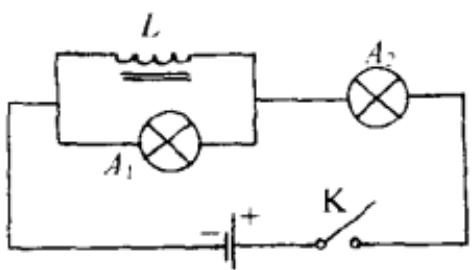
\includegraphics[width=0.5\linewidth]{figures/fig_10_2_1.jpg}
\end{center}
\begin{center}
    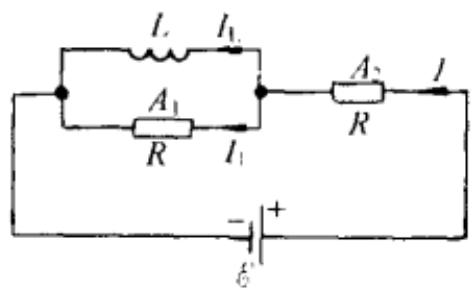
\includegraphics[width=0.5\linewidth]{figures/fig_10_2_2.jpg}
\end{center}

\vfill

\newpage

\textbf{10.3.} 一电路如图 10.3(1)，其中 $S_{1}$ 和 $S_{2}$ 是两个相同的小灯泡，自感为 L 的线圈其电阻也是 R。当开关 K 接通时，两个小灯泡：(1) $S_{1}$ 先比 $S_{2}$ 暗，然后趋于同样亮；(2) $S_{2}$ 先比 $S_{1}$ 暗，然后趋于同样亮；(3) $S_{1}$ 和 $S_{2}$ 同样亮，亮度不变；(4) $S_{1}$ 和 $S_{2}$ 都是先暗后亮，两者始终一样亮。试问上述(1)至(4)四种描述，其中哪个是对的？

【解答】其中(2)是对的.分析如下:设 $S_{1}$ 和 $S_{2}$ 的电阻均为 r, 流过 $S_{1}$ 的电流为 $I_{1}$ , 流过


图10.3(1)
图10.3(2)

$S_{2}$ 的电流为 $I_{2}$ ，流过 L 的电流为 $I_{L}$ ，如图 10.3(2) 所示。则由基尔霍夫电路定律有

$$
r I _ {1} + \varepsilon_ {L} - R I _ {L} = 0\tag{1}
$$

$$
r I _ {2} - R (I - I _ {2}) = 0\tag{2}
$$

$$
I _ {1} + I _ {L} = I\tag{3}
$$

$$
r I _ {1} + r I _ {2} = \xi\tag{4}
$$

式中 $\varepsilon$ 为电源的电动势. 自感 L 的自感电动势为

$$
\varepsilon_ {L} = - L \frac {\mathrm{d} I _ {L}}{\mathrm{d} t}\tag{5}
$$

由式(1)、(5)得

$$
L \frac {\mathrm{d} I _ {L}}{\mathrm{d} t} + R I _ {L} - r I _ {1} = 0\tag{6}
$$

由式(2)、(3)、(4)消去 I 和 $I_{2}$ 得

$$
I _ {1} = \frac {(R + r) \xi}{r (2 R + r)} - \frac {R}{2 R + r} I _ {L}\tag{7}
$$

代入式(6)得

$$
\frac {\mathrm{d} I _ {L}}{\mathrm{d} t} = \frac {2 R (R + r)}{(2 R + r) L} \left[ \frac {\varepsilon}{2 R} - I _ {L} \right]\tag{8}
$$

利用初始条件，K接通时 $(t = 0), I_{L} = 0$ ，解式(8)得

$$
I _ {L} = \frac {\xi}{2 R} (1 - \mathrm{e} ^ {- \frac {R ^ {\prime}}{L} t})\tag{9}
$$

式中

$$
R ^ {\prime} = \frac {2 R (R + r)}{2 R + r}\tag{10}
$$

将式(9)代入式(7)得

$$
I _ {1} = \frac {\varepsilon}{2 r} + \frac {\varepsilon}{2 (2 R + r)} \mathrm{e} ^ {- \frac {R}{L} t}\tag{11}
$$

将式(11)代入式(4)得

$$
I _ {2} = \frac {\varepsilon}{2 r} - \frac {\varepsilon}{2 (2 R + r)} \mathrm{e} ^ {- \frac {R}{L} t}\tag{12}
$$

由式(11)和(12)可见， $t=0$ (K刚接通)时， $I_{1}>I_{2}$ ，所以 $S_{2}$ 先比 $S_{1}$ 暗。当 $t\to\infty$ 时， $I_{1}=I_{2}=\frac{t}{2r}$

$I_{1}$ 和 $I_{2}$ 与时间 t 的关系如图 10.3(3) 所示, 图中 $\Delta=\frac{\varepsilon}{2(2R+r)}$ .

图10.3(3)
\begin{center}
    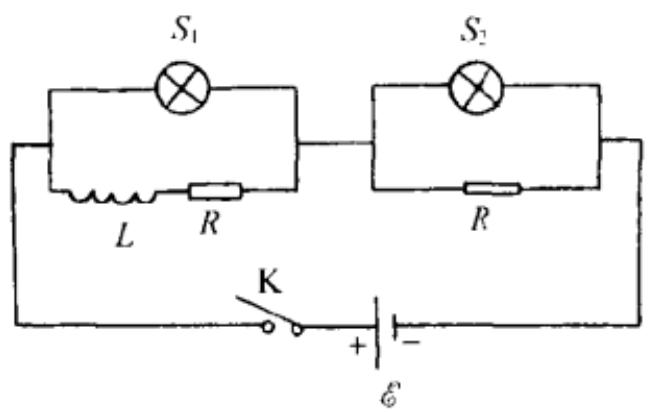
\includegraphics[width=0.5\linewidth]{figures/fig_10_3_1.jpg}
\end{center}
\begin{center}
    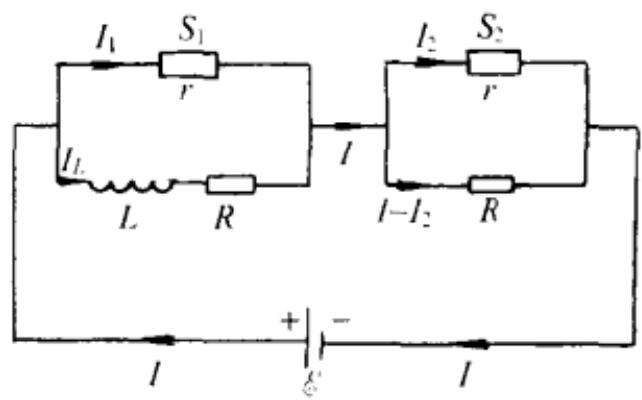
\includegraphics[width=0.5\linewidth]{figures/fig_10_3_2.jpg}
\end{center}
\begin{center}
    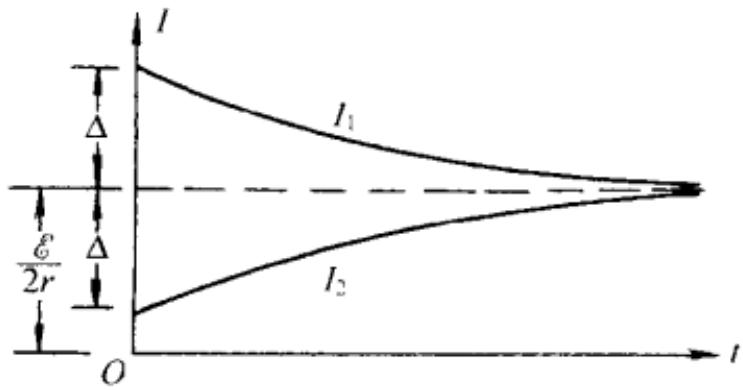
\includegraphics[width=0.5\linewidth]{figures/fig_10_3_3.jpg}
\end{center}

\vfill

\textbf{10.4.} 电阻为 $R_{1}$ 的小灯泡 $S$ 与自感为 $L$ 、电阻为 $R_{2}$ 的线圈并联后，接到电动势为 $\varepsilon$ 、内阻为 $r$ 的电源上，如图10.4(1)所示。接通开关K，使小灯泡稳定地发光。为了使K断开时，小灯泡闪亮一下再熄灭，所需的条件是： $(1)R_{1} > r;(2)R_{2} > r;(3)R_{1} > R_{2};(4)R_{2} > R_{1}$ 。试问其中哪个是对的？

图10.4(1)

图10.4(2)

【解答】其中 $(3)R_{1} > R_{2}$ 是对的.说明如下：K接通后小灯泡稳定地发光时，通过小灯泡的电流为

$$
I _ {1} = \frac {R _ {2}}{R _ {1} + R _ {2}} I = \frac {R _ {2} \varepsilon}{R _ {1} r + R _ {2} r + R _ {1} R _ {2}}\tag{1}
$$

通过 $R_{2}$ 的电流为

$$
I _ {2} = \frac {R _ {1}}{R _ {1} + R _ {2}} I = \frac {R _ {1} \varepsilon}{R _ {1} r + R _ {2} r + R _ {1} R _ {2}}\tag{2}
$$

K 断开后, 如图 10.4(2), 由基尔霍夫电路定律有

$$
I _ {1} + I _ {2} = I = 0\tag{3}
$$

$$
I _ {1} R _ {1} - I _ {2} R _ {2} + \varepsilon_ {L} = 0\tag{4}
$$

其中

$$
\varepsilon_ {L} = - L \frac {\mathrm{d} I _ {2}}{\mathrm{d} t}\tag{5}
$$

由式(2)、(3)、(4)得

$$
\frac {\mathrm{d} I _ {2}}{\mathrm{d} t} = - \frac {R _ {1} + R _ {2}}{L} I _ {2}\tag{6}
$$

利用初始条件 t=0 时， $I_{2}$ 由式(2)表示，解式(6)得

$$
I _ {2} = \frac {R _ {1} c}{R _ {1} r + R _ {2} r + R _ {1} R _ {2}} \mathrm{e} ^ {- \frac {R _ {1} + R _ {2}}{L} t}\tag{7}
$$

由式(3)、(7)得

$$
I _ {1} = - \frac {R _ {1} ^ {\ell}}{R _ {1} r + R _ {2} r + R _ {1} R _ {2}} \mathrm{e} ^ {\frac {R _ {1} + R _ {2}}{L}},\tag{8}
$$

式中负号表示这时 $I_{1}$ 的方向与图 10.4(2) 所示的方向相反.

要使 K 断开时，小灯泡闪亮一下再熄灭，由式(1)、(8)可见，即 t=0 时，

$$
\mid I _ {1} \mid = \frac {R _ {1} \varepsilon}{R _ {1} r + R _ {2} r + R _ {1} R _ {2}} > \frac {R _ {2} \varepsilon}{R _ {1} r + R _ {2} r + R _ {1} R _ {2}}\tag{9}
$$

所以

$$
R _ {1} > R _ {2}\tag{10}
$$
\begin{center}
    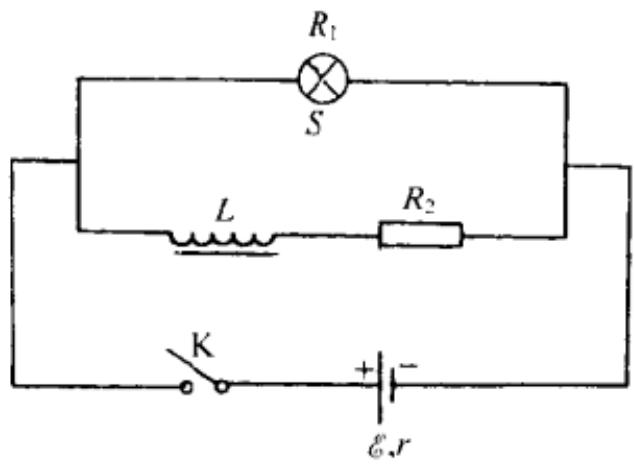
\includegraphics[width=0.5\linewidth]{figures/fig_10_4_1.jpg}
\end{center}
\begin{center}
    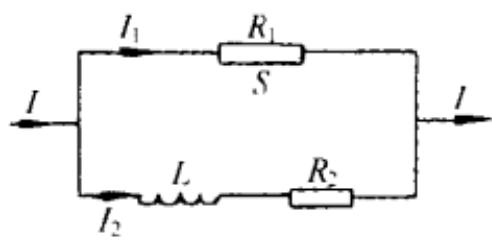
\includegraphics[width=0.5\linewidth]{figures/fig_10_4_2.jpg}
\end{center}

\vfill

\newpage

\textbf{10.5.} 一电路如图 10.5, 其中电感 $L = 200 \mathrm{mH}$ , 电阻 $R = 18 \Omega$ , 电源的电动势为 $\varepsilon = 100 \mathrm{~V}$ , 内阻为 $r = 2 \Omega$ . 在 $t = 0$ 时接通电键 K. 试分别求 $t = 0$ 和 $t = 1.0 \times 10^{-2} \mathrm{~s}$ 时的电流 $I$ , 电流的变化率 $\frac{\mathrm{d} I}{\mathrm{d} t}$ 和电势差 $U_{ab}$ .

\vfill

\textbf{10.6.} 一电报发报机的电路如图 10.6 所示, 仪器 A 由电源 $\varepsilon_{2}$ 供电, 它的开关是继电器 P; 而 P 则由另一电路操纵, 这电路电源的电动势为 $\varepsilon_{1}=20V$ , 总电阻为 $R=80\Omega$ ，自感为 L=0.60H。使继电器 P 的电磁铁工作（即 P 把 $\varepsilon_{2}$ 接通）所需的电流是 $I_{1}\geqslant0.20A$ 。试问 K 接通后，需要多长时间 P 才能接通 $\varepsilon_{2}$ ?
\begin{center}
    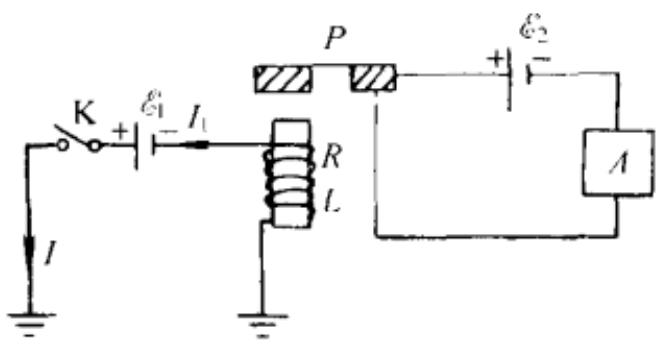
\includegraphics[width=0.5\linewidth]{figures/fig_10_6.jpg}
\end{center}

\vfill

\newpage

\textbf{10.7.} 一个线圈的自感为 L = 3.0H, 电阻为 R = 6.0Ω, 接到电动势为 $\varepsilon = 12V$ 的电源上, 电源的内阻可略去不计. 试求下列时刻的 $\frac{dI}{dt}$ : (1) 刚接上电源; (2) 接上电源后 0.20s; (3) I = 1.0A 时.
\begin{center}
    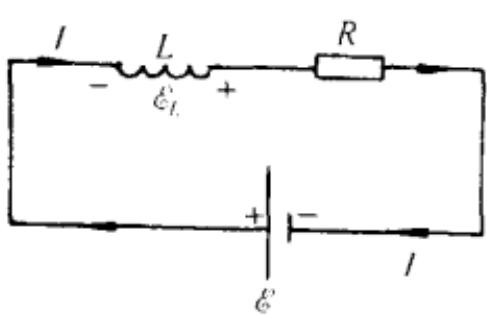
\includegraphics[width=0.5\linewidth]{figures/fig_10_7.jpg}
\end{center}

\vfill

\textbf{10.8.} 一螺线管的自感为 L = 5.0H, 电阻为 R = 20Ω, 在 t = 0 时刻, 将它接到电动势为 $\varepsilon = 100V$ 的电源上, 电源的内阻可略去不计. 试求: (1) 电流 I 与时间 t 的关系; (2) 电流达到稳定值 (不随时间变化的值) 的一半所需要的时间.
\begin{center}
    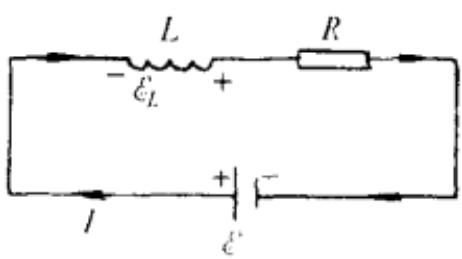
\includegraphics[width=0.5\linewidth]{figures/fig_10_8.jpg}
\end{center}

\vfill

\newpage

\textbf{10.9.} 一电路如图 10.9, 其中的电阻 $R_{1}$ 和 $R_{2}$ , 电感 $L$ 和电动势 $\varepsilon$ 均为已知, 电源的内阻可略去不计. 先接通 $\mathbf{K}_{\mathrm{l}}$ , 使电流 $I$ 达到稳定值. 在 $t = 0$ 时刻接通 $\mathbf{K}_{2}$ . (1) 试求电流 $I$ 与时间 $t$ 的关系; (2) 当 $\varepsilon = 5.0\mathrm{V}, R_{1} = 2.0\Omega, R_{2} = 3.0\Omega, L = 2.0\mathrm{mH}$ 时, 试计算 $t = 1.0 \times 10^{-3}\mathrm{s}$ 时 $I$ 的值.

\vfill

\textbf{10.10.} 一电路如图 10.10(1)，其中电阻 R 和 r，线圈的自感 L 以及电源的电动势 $\varepsilon$ 都已知，电源 $\varepsilon$ 和线圈 L 的内阻都可略去不计。(1)试求开关 K 接通后，a、b 间的电压与时间的关系；(2)在电流达到稳定值的情况下，试求 K 断开后，a、b 间的电压与时间的关系。

\vfill

\newpage

\textbf{10.11.} 一电路如图 10.11, 其中电阻 R 和 r, 线圈的自感 L 以及电源的电动势 $\varepsilon$ 均为已知, 电源的内阻已包括在 r 内, 线圈的电阻可略去不计. 先接通 K, 使电流达到稳定值. 然后在 t=0 时刻断开 K. (1) 试求 R 上的电流 I 与时间 t 的关系；(2)试证明：消耗在 R 上的焦耳热等于开始时储藏在 L 中的磁能.

\vfill

\textbf{10.12.} 一电路如图 10.12(1)，其中电阻 R、线圈的自感 L 以及电源的电动势 $\varepsilon$ 和内阻 r 均为已知，线圈的电阻可略去不计。接通 K 使电流达到稳定值，然后断开 K。试求 K 刚断开时：(1)a、b 间的电势差 $U_{ab}$ ；(2)通过 R 的电流 $I_{R}$ 。

\vfill

\newpage

\textbf{10.13.} 一电路如图 10.13(1)，其中电阻 $R_{1}$ 、 $R_{2}$ 和 $R_{3}$ ，线圈的电感 L 以及电源的电动势 $\varepsilon$ 均为已知，电源的内阻包括在 $R_{1}$ 内，线圈的电阻包括在 $R_{3}$ 内。(1) 在 t=0 时刻接通电键 K，试分别求 $R_{1}$ 、 $R_{2}$ 和 $R_{3}$ 中的电流与时间 t 的关系；(2) K 接通后，待电流达到稳定值，再断开 K。以 K 断开时为 $t'=0$ ，试求 $R_{1}$ 、 $R_{2}$ 和 $R_{3}$ 中的电流与时间 $t'$ 的关系。


图 10.13(1)
图10.13(2)
\begin{center}
    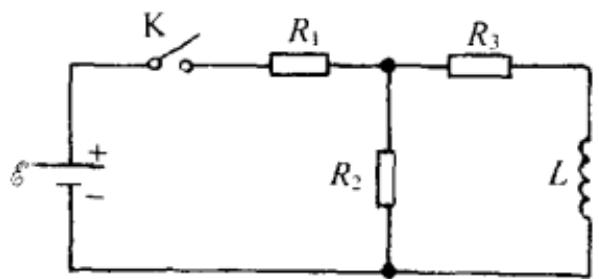
\includegraphics[width=0.5\linewidth]{figures/fig_10_13_1.jpg}
\end{center}
\begin{center}
    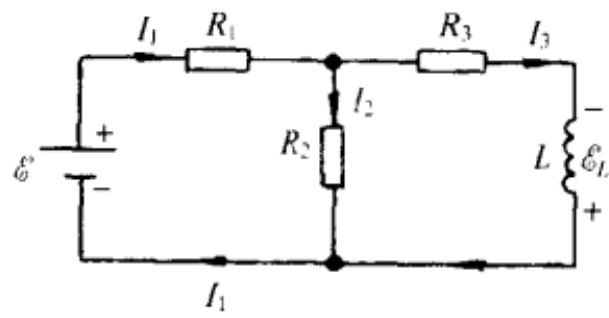
\includegraphics[width=0.5\linewidth]{figures/fig_10_13_2.jpg}
\end{center}

\vfill

\textbf{10.14.} 一电路如图 10.14(1)，其中电阻 R 和 r、线圈的自感 L 和电源的电动势 $\varepsilon$ 都已知，线圈的电阻和电源的内阻都可略去不计。在 t=0 时刻接通开关 K。设 R>r，试求 R 两端的电势差 $U_{R}$ 等于 r 两端的电势差 $U_{r}$ 的时刻。

图10.14(1)

图10.14(2)
\begin{center}
    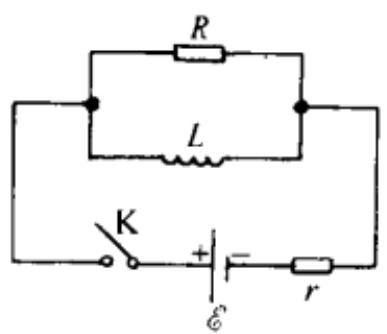
\includegraphics[width=0.5\linewidth]{figures/fig_10_14_1.jpg}
\end{center}
\begin{center}
    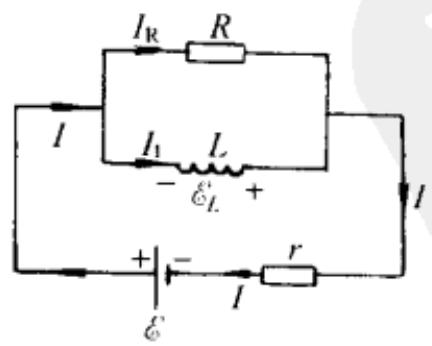
\includegraphics[width=0.5\linewidth]{figures/fig_10_14_2.jpg}
\end{center}

\vfill

\newpage

\textbf{10.15.} 一电路如图 10.15(1)，其中电阻 R、线圈的自感 $L_{1}$ 和 $L_{2}$ 、电源的电动势 $\varepsilon$ 均为已知，线圈的电阻和它们间的互感以及电源的内阻均可略去不计。在$t = 0$ 时刻接通开关K.试求 $t$ 时刻：(1) $a,b$ 间的电势差 $U_{ab}$ ;(2) $L_{1}$ 中的电流 $I_{1}$

图10.15(1)

图10.15(2)
\begin{center}
    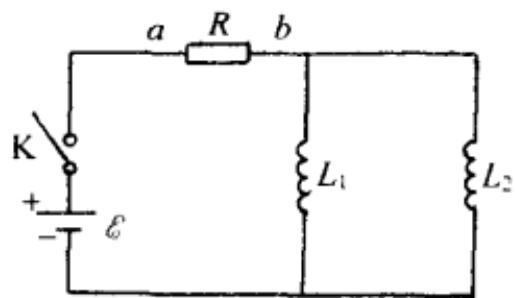
\includegraphics[width=0.5\linewidth]{figures/fig_10_15_1.jpg}
\end{center}
\begin{center}
    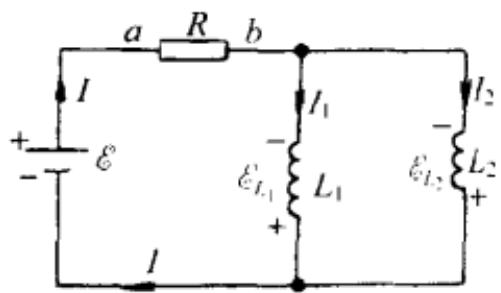
\includegraphics[width=0.5\linewidth]{figures/fig_10_15_2.jpg}
\end{center}

\vfill

\textbf{10.16.} 一电路如图 10.16(1)，已知电源的电动势为 $\varepsilon=220V$ ，内阻可略去不计；线圈的自感为 L=10H，电阻可略去不计；两电阻分别为 $R_{1}=10\Omega$ 和 $R_{2}=100\Omega$ 。(1) 接通开关 K 并持续很长时间，试求这段时间内 $R_{2}$ 上放出的焦耳热；(2) 然后断开 K 并持续很长时间，试求这段时间内 $R_{2}$ 上放出的焦耳热。

图10.16(1)

图10.16(2)
\begin{center}
    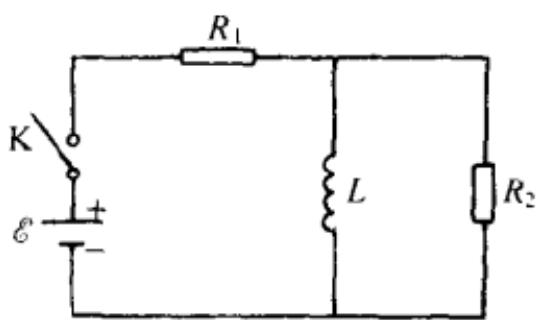
\includegraphics[width=0.5\linewidth]{figures/fig_10_16_1.jpg}
\end{center}
\begin{center}
    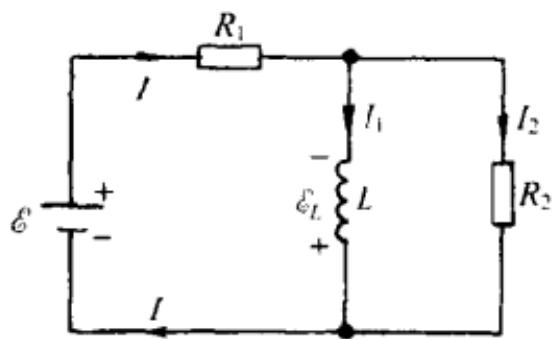
\includegraphics[width=0.5\linewidth]{figures/fig_10_16_2.jpg}
\end{center}

\vfill

\newpage

\textbf{10.17.} 一电路如图10.17,其中电阻 $R_{1}$ 和 $R_{2}$ 线圈的自感 $L$ 和电源的电动势 $\varepsilon$ 均为已知,线圈的电阻可略不计,电源的内阻已包括在 $R_{1}$ 内.在开关 $\mathbf{K}_2$ 断开的情况下,于 $t = 0$ 时刻接通开关 $\mathbf{K}_1$ ,然后在 $t_1$ 时刻接通开关 $\mathbf{K}_2$ .试求 $t(>t_1)$ 时刻 $a,b$ 两点的电势差 $U_{ab}$ .
\begin{center}
    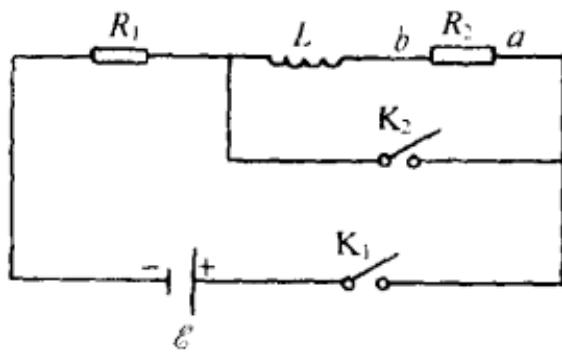
\includegraphics[width=0.5\linewidth]{figures/fig_10_17.jpg}
\end{center}

\vfill

\textbf{10.18.} 一电路如图 10.18, $R_{1}$ 与 $L_{1}$ 串联, $R_{2}$ 与 $L_{2}$ 串联,然后再把它们并联.一电容 C 通过这并联电路放电.试证明:通过这两条支路的电荷量与电阻成反比,即 $Q_{1}/Q_{2}=R_{2}/R_{1}$ .

$$
L _ {1} \frac {\mathrm{d} I _ {1}}{\mathrm{d} t} + R _ {1} I _ {1} = L _ {2} \frac {\mathrm{d} I _ {2}}{\mathrm{d} t} + R _ {2} I _ {2}
$$

\vfill

\newpage

\textbf{10.19.} 一电路如图 10.19, 其中电阻 $R_{1}, R_{2}$ 和 $r$ , 自感 $L_{1}$ 和 $L_{2}$ , 电动势 $\varepsilon$ 均为已知; 电源的内阻已包括在 $r$ 内, $L_{1}$ 和 $L_{2}$ 之间的互感可略去不计. 在 $t = 0$ 时刻接通开关 K, 试求 $t$ 时刻通过电阻 $r$ 的电流 I.

\vfill

\textbf{10.20.} 图 10.20 中有两种电路(1)和(2)，它们的电源内阻都可略去不计。试分析下列四种情况下，哪种情况的自感电动势大于电源的电动势 $\varepsilon$ ：(a) $K_{1}$ 接通时；(b) $K_{1}$ 接通很久后断开时；(c) $K_{2}$ 接通时；(d) $K_{2}$ 接通很久后断开时。

\vfill

\newpage

\textbf{10.21.} 电容为 C 的电容器储有电荷量 $Q_{0}$ ，在 t=0 时刻，接到自感为 L、电阻为 R 的线圈上放电，R 可看作与 L 串联。(1)试求放电电流 I 与时间 t 的关系；

(2)在什么情况下 $I$ 只往一个方向流动？(3)当 $C = 1.0\mu \mathrm{F}, L = 1.6\mathrm{mH}$ 时， $R$ 的值应为多少才满足上述条件？

\vfill

\textbf{10.22.} 一电路如图 10.22, 其中电阻 R、电容 C 和电源的电动势均为已知, C 原来不带电. 试求刚接通电键 K 时, 线路中的电流 I 和 R 两端的电压 $U_{R}$ .

\vfill

\newpage

\textbf{10.23.} 一个 $C = 1.0$ 微法的电容器, 储有能量 $W = 0.50$ 焦耳, 现在让它通过 $R = 1.0 \times 10^{6}$ 欧姆的电阻放电. 试求: (1) 放电前电容器上所容的电荷量 $Q_{0}$ ; (2) 开始放电 $(t = 0)$ 时的电流 $I_{0}$ ; (3) $t$ 时刻电容器上的电压 $U_{C}(t)$ 和 $R$ 上的电压 $U_{R}(t)$ ; (4) $t$ 时刻 $R$ 所消耗的功率 $P(t)$ .

\vfill

\textbf{10.24.} 一电容器的 C 为 $5.0 \mu F$ ，两极板间的介质不是完全绝缘的，因而有漏电电阻，其值为 $2.0 \times 10^{8} \Omega$ 。这电容器原来不带电，在 t = 0 时刻，将它的两极板分别接到一恒流电源的两极上，恒流为 I = 3.0 mA。（1）试求两极板的电势差 U 与时间 t 的关系；（2）试问经过多长时间，U = 500 V？

(1)

(2)
\begin{center}
    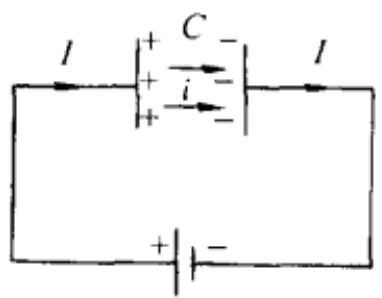
\includegraphics[width=0.5\linewidth]{figures/fig_10_24_1.jpg}
\end{center}
\begin{center}
    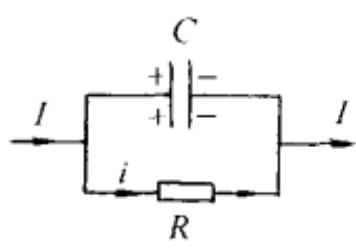
\includegraphics[width=0.5\linewidth]{figures/fig_10_24_2.jpg}
\end{center}

\vfill

\newpage

\textbf{10.25.} 一平行板电容器两极板间充满均匀介质,这介质的电容率为 $\varepsilon$ ,电导率为 $\sigma$ .将这电容器充电,试问断开电源后经过多长时间,它的电荷量或电压降到初值的 $e^{-1} = \frac{1}{2.71828}$ 倍? (这段时间称为弛豫时间)

\vfill

\textbf{10.26.} 一电路如图 10.26, 其中电容 C 和电阻 R 以及电源的电动势 $\delta$ 和内阻 r 均为已知. 接通电链 K, 待电流达到稳定值后, 于 t=0 时刻断开 K. 试求 t 时刻 C 上的电荷量 Q 和通过 R 的电流 I.

\vfill

\newpage

\textbf{10.27.} 一电路如图 10.27, 电容 C 与电阻 R 并联, 接到电动势为 $\varepsilon$ 、内阻为 r 的电源上. 在 t=0 时刻接通电键 K. 试求 t 时刻的 (1) 通过电源的电流 I; (2) R 两端的电压 $U_{R}$ .

\vfill

\textbf{10.28.} 一电路如图 10.28, 电容 $C_{1}$ 和 $C_{2}$ 及电阻 $R_{1}$ 和 $R_{2}$ 均为已知, G 是电流计. 试证明: 如果 $R_{1}C_{1}=R_{2}C_{2}$ , 则接通电键 K 后, G 不会发生偏转.

\vfill

\newpage

\textbf{10.29.} 在 LC 振荡回路中, 设开始 $(t=0)$ 时 C 上的电荷量为 $Q_{0}, L$ 中的电流为零. (1) 试求 L 中的磁场能量第一次等于 C 中的电场能量的时间 $t_{1}$ ; (2) 试求这时 C 上的电荷量 $Q_{1}$ ; (3) 当 $L=10mH, C=1.0\mu F$ 时, 试计算 $t_{1}$ 的值.

\vfill

\textbf{10.30.} 一电路如图 10.30(1), $C_1 = 100\mu \mathrm{F}, C_2 = 900\mu \mathrm{F}, L = 10\mathrm{H}$ . $C_2$ 已充电到 $100\mathrm{V}, C_1$ 未充电. 试问怎样利用电键 $\mathbf{K}_1$ 和 $\mathbf{K}_2$ , 使 $C_1$ 充电到 $300\mathrm{V}$ ?


图10.30(1)
图10.30(2)
\begin{center}
    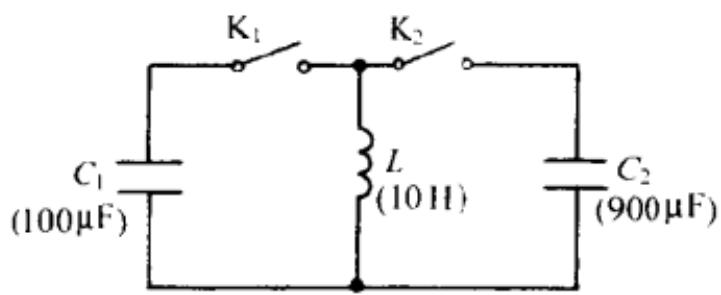
\includegraphics[width=0.5\linewidth]{figures/fig_10_30_1.jpg}
\end{center}
\begin{center}
    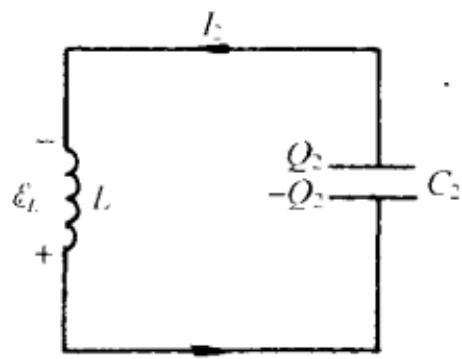
\includegraphics[width=0.5\linewidth]{figures/fig_10_30_2.jpg}
\end{center}

\vfill

\newpage

\textbf{10.31.} 在电阻 $R = 5\Omega$ ，电感 $L = 10mH$ ，电容 $C = 10\mu F$ 的串联电路两端，加上频率为 $f = 50Hz$ 的简谐交流电压，试问经过该交流电的几个周期后，暂态过程的电流便小于开始后最大值的百分之一？

\vfill

\textbf{10.32.} $R = 1000\Omega, L = 0.10\mathrm{H}, C = 0.010\mu \mathrm{F}$ , 串联如图 10.32(1)所示. 先使 $C$ 充电到 400 伏特, 在 $t = 0$ 时接通电键 K. (1)试求电路中电流 $I$ 与时间 $t$ 的关系; (2)在第一个振荡周期里有多少能量变为焦耳热? (3)在全部振荡时间内有多少能量变为焦耳热? (4)电路中应串入多大电阻, 才能使它不发生振荡?

图10.32(1)

图10.32(2)
\begin{center}
    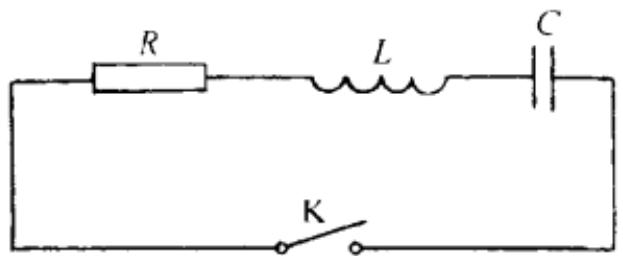
\includegraphics[width=0.5\linewidth]{figures/fig_10_32_1.jpg}
\end{center}
\begin{center}
    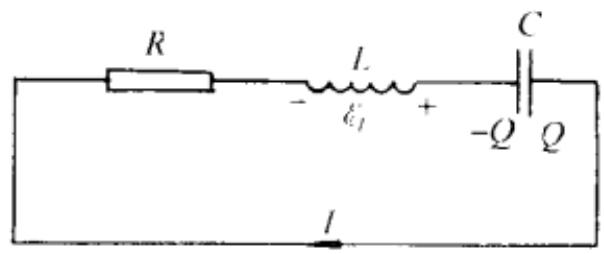
\includegraphics[width=0.5\linewidth]{figures/fig_10_32_2.jpg}
\end{center}

\vfill

\newpage

\textbf{10.33.} 两电容 $C_1$ 和 $C_2$ , 各有一极板接地. 开始时, $C_1$ 上有电荷量 $Q_0, C_2$ 不带电, 它们与已知的电阻 $R$ 和自感 $L$ 联接如图 10.33 所示. 在 $t = 0$ 时接通开关 K. 试证明: 若 $R^2 = 4L\left(\frac{1}{C_1} + \frac{1}{C_2}\right)$ , 则在 $t = 2L / R$ 时刻通过 $R$ 的电流为极大, 其值为 $I_m = \frac{2Q_0}{\mathrm{e}RC_1}$ , 式中 e 是自然对数的底.
\begin{center}
    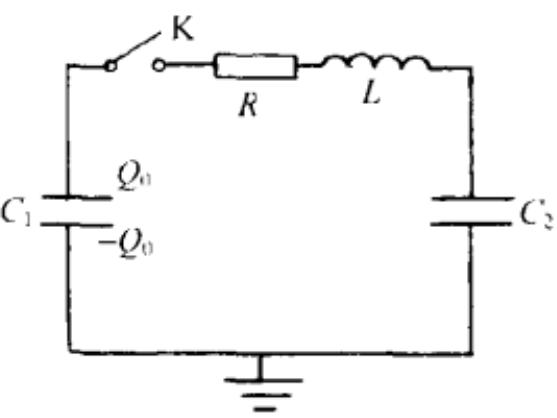
\includegraphics[width=0.5\linewidth]{figures/fig_10_33.jpg}
\end{center}

\vfill

\textbf{10.34.} 电阻 R、电感 L 和电容 C 串联电路的谐振角频率为 $\omega_{0}$ ，R 和 L 串联电路的时间常数为 $\tau_{RL}$ ，R 和 C 串联电路的时间常数为 $\tau_{RC}$ 。试求 $\omega_{0}$ 、 $\tau_{RL}$ 和 $\tau_{RC}$ 三者间的关系。


图10.34(1)
图 10.34(2)
\begin{center}
    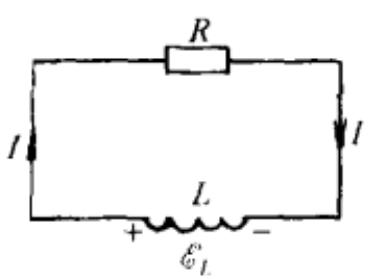
\includegraphics[width=0.5\linewidth]{figures/fig_10_34_1.jpg}
\end{center}
\begin{center}
    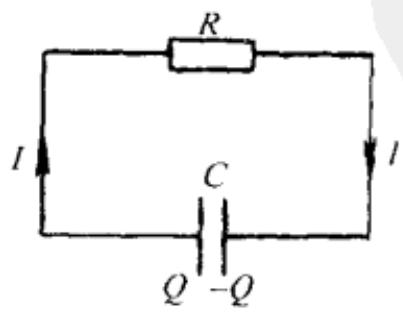
\includegraphics[width=0.5\linewidth]{figures/fig_10_34_2.jpg}
\end{center}

\vfill

\newpage

\textbf{10.35.} 一 RLC 串联电路, 开始时电容 C 带有电荷量 $Q_{0}$ , 如图 10.35(1) 所示. 接通开关 K 后, C 便经过 RL 放电. 因 $R < 2\sqrt{L/C}$ , 电流发生振荡. 试求一个周期里损失的能量 $\Delta\overline{W}$ 与该周期开始时电路里所储存的能量 $\overline{W}$ 之比 $\Delta\overline{W}/\overline{W}$ .


图10.35(1)
图 10.35(2)
\begin{center}
    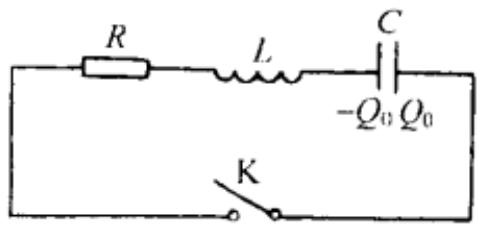
\includegraphics[width=0.5\linewidth]{figures/fig_10_35_1.jpg}
\end{center}
\begin{center}
    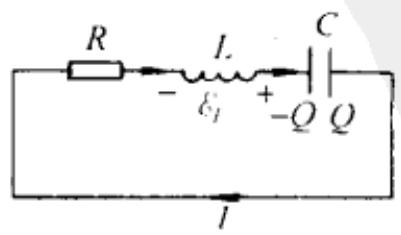
\includegraphics[width=0.5\linewidth]{figures/fig_10_35_2.jpg}
\end{center}

\vfill

\textbf{10.36.} 一电路如图 10.36(1)，接通开关 K 后，电容 C 经两条支路放电。设 Q 为 C 上的电荷量。试证明

$$
\begin{array}{l} R ^ {\prime} L \frac {\mathrm{d} ^ {3} Q}{\mathrm{d} t ^ {3}} + \left(R R ^ {\prime} + \frac {L}{C} + \frac {L}{C ^ {\prime}}\right) \frac {\mathrm{d} ^ {2} Q}{\mathrm{d} t ^ {2}} \\ + \left(\frac {R}{C} + \frac {R}{C ^ {\prime}} + \frac {R ^ {\prime}}{C}\right) \frac {\mathrm{d} Q}{\mathrm{d} t} + \frac {Q}{C C ^ {\prime}} = 0 \end{array}
$$

图10.36(1)

图 10.36(2)
\begin{center}
    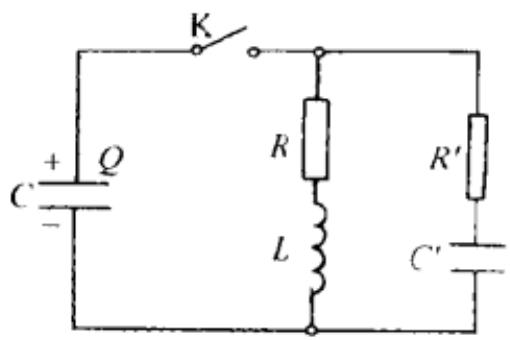
\includegraphics[width=0.5\linewidth]{figures/fig_10_36_1.jpg}
\end{center}
\begin{center}
    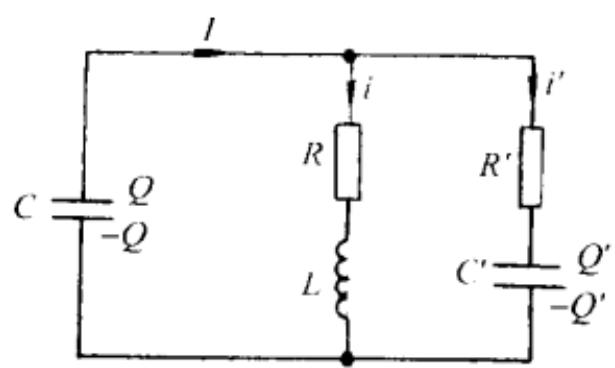
\includegraphics[width=0.5\linewidth]{figures/fig_10_36_2.jpg}
\end{center}

\vfill

\newpage

\textbf{10.37.} 两线圈 $L_{1}$ 和 $L_{2}$ 的电阻分别为 $R_{1}$ 和 $R_{2}$ , 它们之间的互感为 $M$ ; 第一个线圈接在电动势为 $\varepsilon$ 的电源上 (电源的内阻可略去不计), 第二个线圈接在电阻为 $R_{g}$ 的电流计 G 上, 如图 10.37 所示. 电键 K 原先是接通的, 第一个线圈内电流已达到稳定. 设在 $t = 0$ 时断开 K, 试求流过电流计的电流 $I_{2}$ 和电荷量 Q.
\begin{center}
    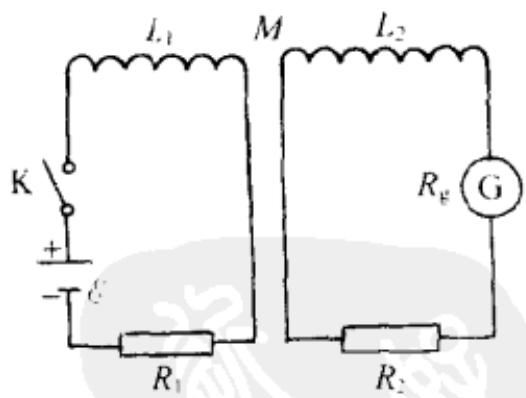
\includegraphics[width=0.5\linewidth]{figures/fig_10_37.jpg}
\end{center}

\vfill

\textbf{10.38.} 一质量为 $m$ 的物体，在弹性力 $-kx$ 、阻尼力 $-\alpha \frac{\mathrm{d}x}{\mathrm{d}t}$ 和策动力 $F_0 \cos \omega t$ 的作用下，在 $x$ 轴上振动；由于运动方程(微分方程)相似，可以用 $R, L, C$ 串联后加上交流电压 $\mathcal{E} = \mathcal{E}_0 \sin \omega t$ 来模拟它的运动。试求与质量 $m$ 、倔强系数 $k$ 、阻尼系数 $\alpha$ 、策动力的振幅 $F_0$ 、固有频率 $w_0$ 和品质因数等分别相对应的电学量。

\vfill

\newpage

\textbf{10.39.} 如图 10.39, 一平面线圈的面积为 S, 电阻为 R, 自感为 L, 在一个不变的均匀磁场(磁感强度为 B) 中, 从 t=0 时刻开始, 以匀角速度 $\omega$ 绕一固定轴旋转, 转轴与线圈共面, B 与转轴垂直, 且 t=0 时 B 与线圈的平面垂直. 试求 t 时刻线圈中的电流 I.

\vfill
